\documentclass[12pt]{article}
\usepackage[frenchb]{babel} 
\usepackage[T1]{fontenc}
\usepackage[utf8]{inputenc}
%\usepackage{lmodern} 
\usepackage{graphicx}
\usepackage{multirow}
\usepackage[top=2.5cm, bottom=2.5cm, left=2.5cm , right=2.5cm]{geometry}
%\usepackage{amsmath}
%\usepackage{amsthm}
%\usepackage{amsfonts}
\usepackage{empheq}
\usepackage{setspace}
\usepackage{hyperref}
\hypersetup{pdftitle = {INF4215 - Rapport de laboratoire}, pdfauthor={Julien Antoine}}
\usepackage{color}
\usepackage{subfigure}
\usepackage{fancyvrb}
\usepackage{SIunits}
\usepackage{numprint}
\usepackage{enumitem}
\usepackage{calc}
\usepackage{listings}
\usepackage{float}
\usepackage{cellspace}
\cellspacetoplimit=4pt
\cellspacebottomlimit=4pt

% ----------------------------------- FANCY HEADER -----------------------------------
\usepackage{fancyhdr}
\pagestyle{fancy}
\renewcommand{\headrulewidth}{0.5pt}
%\fancyhead[C]{\textbf{page \thepage}} 
\fancyhead[L]{}
\fancyhead[R]{Rapport de laboratoire}

\renewcommand{\footrulewidth}{0.5pt}
\fancyfoot[C]{\textbf{\thepage}} 
\fancyfoot[L]{Polytechnique Montréal}
\fancyfoot[R]{INF4215 -- Intelligence artificielle}
% ------------------------------------------------------------------------------------


\providecommand{\e}[1]{\ensuremath{\cdot 10^{#1}}}
\newcommand{\question}{\noindent$\bullet$\;\;}
\newcommand{\eau}{\ensuremath{\text{H}_2 \text{O}}}
\newcommand{\dio}{\ensuremath{\text{CO}_2}}
%\addto\captionsfrancais{\renewcommand{\chaptername}{Labo}}

\begin{document}

\hyphenation{HyperLogLog experimental techno-logy according develop-ment}


\begin{titlepage}
\newcommand{\HRule}{\rule{\linewidth}{0.5mm}} % Defines a new command for the horizontal lines, change thickness here
\center % Center everything on the page
%------------------------------------------------------------------------------------
%	LOGO SECTION
%------------------------------------------------------------------------------------
\raggedright
\includegraphics[width = 0.33\textwidth]{../../../logo}\\[6cm] 
\centering
%------------------------------------------------------------------------------------
%	TITLE SECTION
%------------------------------------------------------------------------------------
\HRule \\[0.4cm]
{ \huge \bfseries INF4215 -- Rapport de laboratoire}\\[0.4cm]
{ \Large \bfseries Recherche dans un espace d'états}\\%[0.4cm] 
\HRule \\[1cm]
%------------------------------------------------------------------------------------
%	AUTHOR SECTION
%------------------------------------------------------------------------------------
\begin{minipage}{0.45\textwidth}
\begin{center} \large
Julien \textsc{Antoine}\\
1813026
\end{center}
\end{minipage}
~
\begin{minipage}{0.45\textwidth}
\begin{center} \large
Abdelhadi \textsc{Temmar}\\
1805815
\end{center}
\end{minipage}\\[8cm]
%------------------------------------------------------------------------------------
%	DATE SECTION
%------------------------------------------------------------------------------------
\begin{center}
{\large 14 février 2015}
\end{center}
%------------------------------------------------------------------------------------
\vfill % Fill the rest of the page with whitespace
\end{titlepage}



\section{Recherche arborescente}
\subsection{Représentation du problème}
%Chaque état contient la liste des points restant à couvrir, la liste des antennes placées et leur coût total. A l'état initial, on a donc la liste complète des points à couvrir, une liste vide pour les antennes, et un coût de 0.

\subsubsection{Représentation d'un état}
Un état est composé de:
\begin{itemize}
	\item un ensemble comprenant les coordonnées des points restant à couvrir
	\item un ensemble comprenant les antennes placées (position et rayon)
%	\item le coût requis par les antennes déjà placées
\end{itemize}

\subsubsection{Etat initial}
L'état initial est donc composé de l'ensemble des points à couvrir, d'un ensemble vide (représentant les antennes placées), et d'un coût de 0.

\subsubsection{Actions possibles}
Une seule action est possible à partir d'un état: l'ajout d'une nouvelle antenne.
Cependant, avant de chercher les antennes que l'on peut possiblement ajouter, nous vérifions que le nombre d'antennes de l'état ne dépasse pas le nombre de points initiaux et que le coût de l'ajout d'une nouvelle antenne additionné à celui des antennes déjà placées
%$coutActuelEtat + K  + C$ 
ne dépasse pas le coût maximal. En effet, nous ne voulons pas que notre programme retourne une solution avec un coût supérieur à celui qu'on obtiendrait si on ne plaçait qu'une seule antenne couvrant tous les points.

Nous recherchons ensuite la liste des antennes que l'on peut ajouter, toujours en vérifiant que cet ajout n'engendre pas une solution avec un coût supérieur au coût maximal. Si aucun point ne se trouve sur le périmètre maximal de l'antenne, nous décidons de ne pas la considérer. Nous ne voulons pas de rayon trop grand inutilement.


\subsubsection{État final}
Un état est final si l'ensemble de points qu'il reste à couvrir est vide.


\subsection{Type de recherche choisi}
Après plusieurs tests, l'algorithme de recherche en profondeur s'est avéré le plus efficace pour notre recherche arborescente. Il apporte une solution en environ une minute pour une grille de $50 \times 50$ sans qu'on ait à faire aucune vérification particulière sur un n\oe ud après ajout d'une antenne. 

L'algorithme de recherche au moindre de coût ne retourne toujours pas de résultat en 1h de recherche pour une taille de grille de $50 \times 50$.
Nous avons donc essayé d'utiliser l'algorithme A* et de trouver une heuristique capable d'améliorer la recherche de moindre coût. Malheureusement aucune de nos heuristiques n'a donné de résultat concluant.

Il a donc fallu faire un choix entre optimalité et rapidité. N'ayant pas trouvé une façon d'obtenir la solution optimale en moins d'une heure, nous avons préféré opter pour l'algorithme de recherche en profondeur qui garantit de trouver une solution convenable en un minimum de temps.



%\subsection{Recherche en profondeur}
%
%\subsection{Recherche au moindre coût}
%
%\subsection{Recherche A*}


\section{Recherche locale}
Un deuxième type de recherche est la recherche locale. Contrairement à la recherche arborescente vue dans la section précédente, la locale part d'un état et essaie de l'améliorer sur base de satisfaction de contraintes.

\subsection{Représentation du problème}
\subsubsection{Représentation d'un état}
Un état est simplement composé d'une liste des antennes placées (position, rayon et coordonnées des points couverts), par exemple:
\begin{equation*}
	\texttt{[(20,15,7,[(22,19),(14,15),(17,18)])]}
\end{equation*}
signifie qu'une seule antenne est positionnée en $(20,15)$ avec un rayon de taille 7, et qu'elle couvre les points $(22,19)$, $(14,15)$ et $(17,18)$.


\subsubsection{Etat initial}
L'état initial est celui où une antenne de rayon 1 est placée sur chaque point à couvrir.

\subsubsection{Actions possibles}
Les actions possibles à partir de chaque état est une fusion entre deux antennes. Cette action est faisable uniquement si le coût de l'antenne résultante de la fusion de deux antennes est inférieur au coût total des deux antennes. Lors de la fusion, l'antenne résultante se situe au barycentre des points couverts par chacune des deux antennes fusionnées, et a pour rayon la distance entre ce barycentre et le point couvert par l'antenne le plus éloigné.

\subsubsection{Etat final}
L'état final est atteint lorsque plus aucune fusion n'est possible.


\subsection{Résultats}
Cette méthode est considérablement plus rapide que la recherche arborescente, puisque le nombre d'opérations effectuées est bien moindre. Sur une grille de $50 \times 50$, on obtient une solution proche de l'optimale (voir figure \ref{50x50}) en moins d'une milliseconde. Afin d'améliorer la solution, une fois toutes les fusions effectuées, on regarde pour chaque antenne si en la déplaçant dans un voisinage de $5 \times 5$ on peut réduire son rayon tout en continuant de couvrir les points qu'elle couvrait déjà. Cela permet d'améliorer la solution trouvée et de la rapprocher encore plus de l'optimale.

\vspace{0.5cm}
Nous choisissons donc notre implémentation locale pour le concours.

\begin{figure}[H]
  \centering
  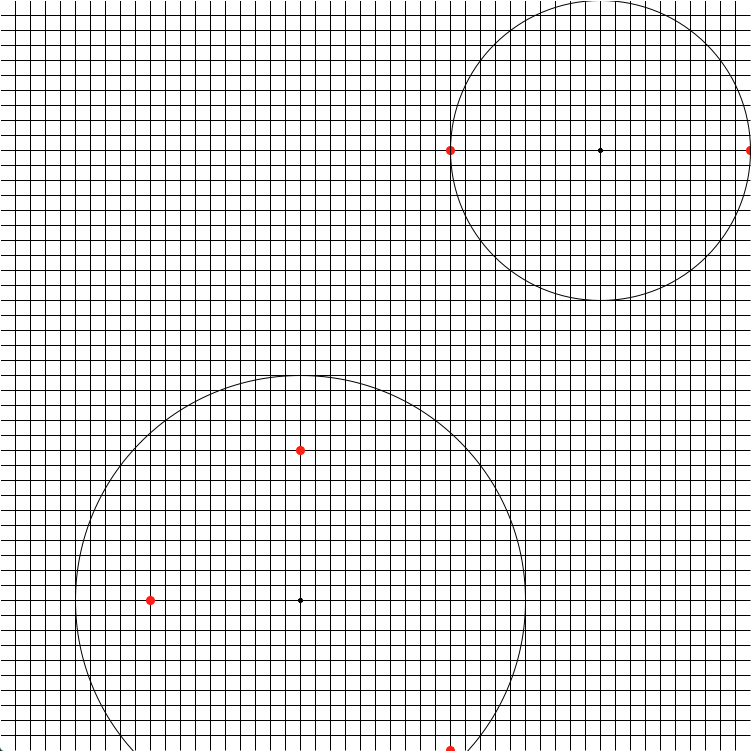
\includegraphics[width = 0.7\textwidth]{50x50}
  \caption{Résultat de la recherche locale pour l'exemple de l'énoncé}
  \label{50x50}
\end{figure}



\section{Réponses aux questions}
\paragraph{a)}
La fonction \texttt{fct} renvoie uniquement les éléments de \texttt{inputList} qui vérifient les prédicats présents dans \texttt{predList}.
Par exemple,
\begin{equation*}
	\texttt{fct([lambda: x < 8, lambda: x > 3], [1,2,3,4,5,6,7,8])}
\end{equation*}
retourne les éléments compris strictement entre 3 et 8, donc [4,5,6,7].


\paragraph{b)}
Le point fort de notre recherche locale est clairement sa rapidité d'exécution. Quelle que soit la taille de la grille ou le nombre de points, elle retourne toujours un résultat endéans la seconde. Le résultat retourné est en général assez proche de l'optimal, on n'obtient jamais de résultat absurde. Sa faiblesse est qu'elle ne retourne jamais la solution optimale, sauf dans certains cas simples comprenant une symétrie par exemple.

Notre recherche arborescente a comme point fort de garantir de trouver la solution optimale. Cependant, ce point est largement contre balancé par le fait que pour des tailles de grilles plus conséquentes, elle ne produit pas de résultat avant au moins 45 minutes. Cela est notamment dû à des lacunes dans l'heuristique, que nous n'avons malheureusement pas réussi à améliorer comme nous l'aurions désiré.











\end{document}
